\chapter[Exemplos]{exemplos}
\label{ch:exemplos}

% EXEMPLO CITACAO INLINE
Seu texto pode conter citacoes como em \cite{Legislativa} ou referenciass a \autoref{fig:rede_convencional}.

% EXEMPLO CITACAO <3 LINHAS
Exemplo de citação direta com menos de três linhas. Como "o mercado de energia elétrica está baseado em tarifas fixas e limitações de informações em tempo real sobre gerenciamento da rede e da carga" \cite[p. 15]{cgee}, o consumidor acaba, então, não tendo como optar por fornecimentos elétricos mais adequados.

% EXEMPLO CITACAO BLOCO
\begin{citacao}[brazil]
[...] redes elétricas que podem, de forma inteligente, integrar o comportamento e as ações de todos os usuários conectados a ela, como geradores, consumidores e os que desempenham as duas funções, para entregar, eficientemente, um fornecimento de eletricidade sustentável, econômico e seguro \cite[p. 51, tradução livre]{yu2011new}.
\end{citacao}

% EXEMPLO L
\lipsum[1-1]

% EXEMPLO LISTAS
Itens em latex:
\begin{itemize}
	\item texto 1;
	\item texto 2;
	\item texto 3;
\end{itemize}

% EXEMPLO FIGURAS
\begin{figure}[h!]
	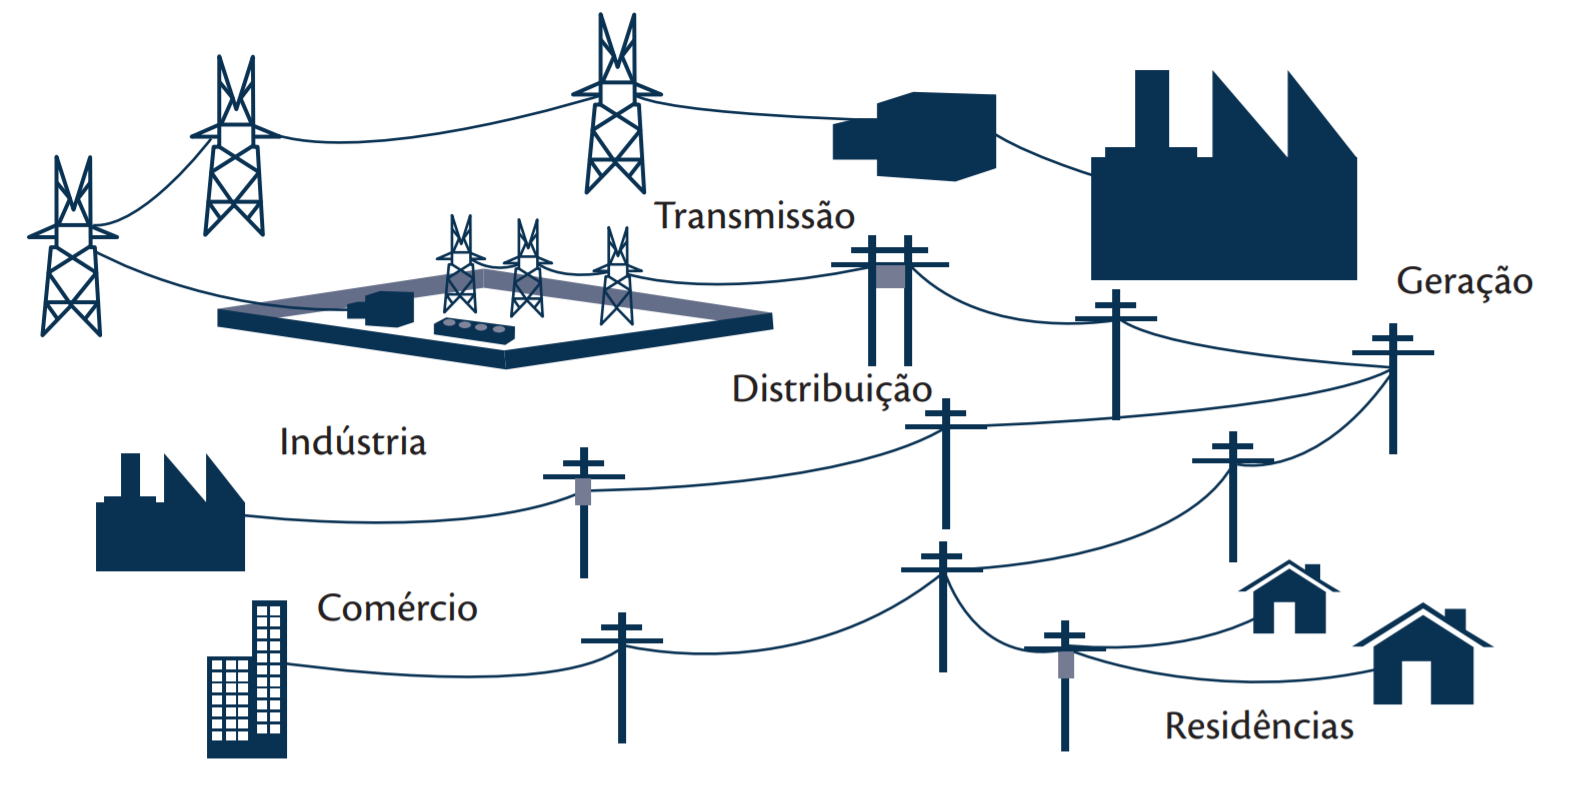
\includegraphics[width=0.9\textwidth, keepaspectratio=true]{rede_convencional}
	\centering
	\caption[Esquemático de uma rede elétrica convencional.]{Esquemático de uma rede elétrica convencional.}
	\fonte{\cite[p. 15]{cgee}.}
	\label{fig:rede_convencional}
\end{figure}
\FloatBarrier

% EXEMPLO TABELAS
\begin{table}[!ht]
    \centering
    \resizebox{\textwidth}{!}{%
    \begin{tabular}{ll}
    \hline
    \multicolumn{1}{c}{\textbf{Redes Elétricas Tradicionais}} &
    \multicolumn{1}{c}{\textbf{Redes Elétricas Inteligentes}} \\
    \hline
    \rowcolor[HTML]{DDDDDD} 
    Eletromecânica, estado sólido                             &
    Digital/Microprocessadores                                \\
    
    Unidirecional e localmente bidirecional                   &
    Global/comunicação bidirecional integrada                 \\
    
    \rowcolor[HTML]{DDDDDD} 
    Geração centralizada                                      &
    Acomoda geração distribuída                               \\
    
    Controle, monitoramento e proteção limitados              &
    WAMPAC, proteção adaptativa                               \\
    
    \rowcolor[HTML]{DDDDDD} 
    "Cega"                                                    & Auto-monitoramento                                        \\
    
    Recuperação manual                                        & Auto-reconfigurável                                       \\
    
    \rowcolor[HTML]{DDDDDD}
    
    Checagem manual de equipamentos                           &
    Monitoração remota de equipamentos                        \\
    
    Sistema de controle de contingências limitado             &
    Sistema de controle pervasivo                             \\
    
    \rowcolor[HTML]{DDDDDD}
    Confiabilidade estimada                                   &
    Confiabilidade preditiva                                   
    \end{tabular}%
    }
    \caption{Comparação entre redes elétricas convencionais e redes elétricas inteligentes}
    \label{tab-comparativa}
    \fonte{\cite[p. 28, tradução nossa]{ali2013smart}}
    \end{table}